% Options for packages loaded elsewhere
\PassOptionsToPackage{unicode}{hyperref}
\PassOptionsToPackage{hyphens}{url}
%
\documentclass[
]{article}
\title{Dungeness River Winter Steelhead SONAR-based Escapement Estimates}
\usepackage{etoolbox}
\makeatletter
\providecommand{\subtitle}[1]{% add subtitle to \maketitle
  \apptocmd{\@title}{\par {\large #1 \par}}{}{}
}
\makeatother
\subtitle{2019 - 2022}
\author{Bethany Craig\textsuperscript{1,*}, Kevin See\textsuperscript{1}, and Joseph Anderson\textsuperscript{1}}
\date{September 08, 2023}

\usepackage{amsmath,amssymb}
\usepackage{lmodern}
\usepackage{iftex}
\ifPDFTeX
  \usepackage[T1]{fontenc}
  \usepackage[utf8]{inputenc}
  \usepackage{textcomp} % provide euro and other symbols
\else % if luatex or xetex
  \usepackage{unicode-math}
  \defaultfontfeatures{Scale=MatchLowercase}
  \defaultfontfeatures[\rmfamily]{Ligatures=TeX,Scale=1}
\fi
% Use upquote if available, for straight quotes in verbatim environments
\IfFileExists{upquote.sty}{\usepackage{upquote}}{}
\IfFileExists{microtype.sty}{% use microtype if available
  \usepackage[]{microtype}
  \UseMicrotypeSet[protrusion]{basicmath} % disable protrusion for tt fonts
}{}
\makeatletter
\@ifundefined{KOMAClassName}{% if non-KOMA class
  \IfFileExists{parskip.sty}{%
    \usepackage{parskip}
  }{% else
    \setlength{\parindent}{0pt}
    \setlength{\parskip}{6pt plus 2pt minus 1pt}}
}{% if KOMA class
  \KOMAoptions{parskip=half}}
\makeatother
\usepackage{xcolor}
\IfFileExists{xurl.sty}{\usepackage{xurl}}{} % add URL line breaks if available
\IfFileExists{bookmark.sty}{\usepackage{bookmark}}{\usepackage{hyperref}}
\hypersetup{
  pdftitle={Dungeness River Winter Steelhead SONAR-based Escapement Estimates},
  pdfauthor={Bethany Craig1,, Kevin See1, and Joseph Anderson1},
  hidelinks,
  pdfcreator={LaTeX via pandoc}}
\urlstyle{same} % disable monospaced font for URLs
\usepackage[margin=1in]{geometry}
\usepackage{longtable,booktabs,array}
\usepackage{calc} % for calculating minipage widths
% Correct order of tables after \paragraph or \subparagraph
\usepackage{etoolbox}
\makeatletter
\patchcmd\longtable{\par}{\if@noskipsec\mbox{}\fi\par}{}{}
\makeatother
% Allow footnotes in longtable head/foot
\IfFileExists{footnotehyper.sty}{\usepackage{footnotehyper}}{\usepackage{footnote}}
\makesavenoteenv{longtable}
\usepackage{graphicx}
\makeatletter
\def\maxwidth{\ifdim\Gin@nat@width>\linewidth\linewidth\else\Gin@nat@width\fi}
\def\maxheight{\ifdim\Gin@nat@height>\textheight\textheight\else\Gin@nat@height\fi}
\makeatother
% Scale images if necessary, so that they will not overflow the page
% margins by default, and it is still possible to overwrite the defaults
% using explicit options in \includegraphics[width, height, ...]{}
\setkeys{Gin}{width=\maxwidth,height=\maxheight,keepaspectratio}
% Set default figure placement to htbp
\makeatletter
\def\fps@figure{htbp}
\makeatother
\setlength{\emergencystretch}{3em} % prevent overfull lines
\providecommand{\tightlist}{%
  \setlength{\itemsep}{0pt}\setlength{\parskip}{0pt}}
\setcounter{secnumdepth}{5}
\newlength{\cslhangindent}
\setlength{\cslhangindent}{1.5em}
\newlength{\csllabelwidth}
\setlength{\csllabelwidth}{3em}
\newlength{\cslentryspacingunit} % times entry-spacing
\setlength{\cslentryspacingunit}{\parskip}
\newenvironment{CSLReferences}[2] % #1 hanging-ident, #2 entry spacing
 {% don't indent paragraphs
  \setlength{\parindent}{0pt}
  % turn on hanging indent if param 1 is 1
  \ifodd #1
  \let\oldpar\par
  \def\par{\hangindent=\cslhangindent\oldpar}
  \fi
  % set entry spacing
  \setlength{\parskip}{#2\cslentryspacingunit}
 }%
 {}
\usepackage{calc}
\newcommand{\CSLBlock}[1]{#1\hfill\break}
\newcommand{\CSLLeftMargin}[1]{\parbox[t]{\csllabelwidth}{#1}}
\newcommand{\CSLRightInline}[1]{\parbox[t]{\linewidth - \csllabelwidth}{#1}\break}
\newcommand{\CSLIndent}[1]{\hspace{\cslhangindent}#1}
\usepackage{fancyhdr}
\usepackage{float}
\usepackage{placeins}
\addtolength{\headheight}{1.0cm}
\pagestyle{fancyplain}
\fancyhead[R]{\includegraphics[height=1.2cm]{../templates/wdfwlogo_clr.png}}
\fancyhead[L]{} \renewcommand{\headrulewidth}{0pt}
\usepackage{booktabs}
\usepackage{longtable}
\usepackage{array}
\usepackage{multirow}
\usepackage{wrapfig}
\usepackage{float}
\usepackage{colortbl}
\usepackage{pdflscape}
\usepackage{tabu}
\usepackage{threeparttable}
\usepackage{threeparttablex}
\usepackage[normalem]{ulem}
\usepackage{makecell}
\usepackage{xcolor}
\ifLuaTeX
  \usepackage{selnolig}  % disable illegal ligatures
\fi

\begin{document}
\maketitle

{
\setcounter{tocdepth}{2}
\tableofcontents
}
\textsuperscript{1} Washington Department of Fish \& Wildlife

\textsuperscript{*} Correspondence: \href{mailto:Bethany.Craig@dfw.wa.gov}{Bethany Craig \textless{}\href{mailto:Bethany.Craig@dfw.wa.gov}{\nolinkurl{Bethany.Craig@dfw.wa.gov}}\textgreater{}}

\newpage

\hypertarget{executive-summary}{%
\section{Executive Summary}\label{executive-summary}}

This report contains methods and results of SONAR-based escapement estimates for winter steelhead on the Dungeness River from 2019-2022. WDFW deployed a multibeam SONAR unit in the lower Dungeness River during the majority of the steelhead return from either early February or early March through the end of June or July, 2018-2022. Although the SONAR was operated in 2018, we were not able to produce a SONAR-based escapement estimate for 2018 due to frequent milling behavior at the site, and limited data review. We initiated a sub-sampling protocol in 2019 to enable us to review the entire season of imagery, and this was continued in subsequent years.

To exclude similarly sized fish that were not steelhead from our SONAR counts, WDFW conducted weekly species composition sampling in 2021 and 2022 throughout the periods of SONAR operation. The majority of fish encountered were steelhead and bull trout and these species overlapped in length up to 67 cm. To exclude potential bull trout from the SONAR fish counts we fit a binomial GAM with a logit link, using splines of fork length and Julian day to predict the probability of a fish being a steelhead for fish measured as 67 cm or less. The probability of being a steelhead was greatest during March and April, and least in February and June when more bull trout were present.

To fill in the missing data from periods when the SONAR was not operating or the data had not been reviewed, we fit the fish count data with a negative binomial generalized additive model (GAM) with a log link function using hour of day, discharge, and Julian day-of-year as covariates. For both upstream and downstream moving fish, the model indicates that a greater number of steelhead will move during the night, especially in the late evening, compared to the daytime, and more will move when discharge flows are near 600 cfs. There is also a clear effect of day-of-year, with upstream numbers peaking near the beginning of April, while downstream numbers peak near the beginning of May, with some year-to-year variability in the run-timing curve.

To generate an annual estimate of escapement, we subtracted the total estimate of downstream moving fish from the total estimate of upstream moving fish prior to May 15th to prevent double counting milling fish. After May 15, we ignored downstream moving fish and only estimated upstream moving fish, under the assumption that downstream moving fish are steelhead kelts that have spawned and therefore should not be subtracted from our escapement estimates. Total SONAR-based escapement estimates for steelhead ranged from 646 (CI 626 -- 668) in 2021 to 1,101 (CI 1012 -- 1196) in 2020. The SONAR-based estimates were consistently roughly twice the redd-based estimates.

We learned some important lessons over the first 5 years of SONAR operation on the Dungeness River. Site selection is important and may need to change if fish aren't actively migrating past the site. For future seasons we recommend deploying the SONAR in January, to capture the start of the steelhead return. We also recommend considering re-designing the species composition sampling to attempt to exclude holding fish, and to investigate how species composition changes with hour of day, since returning steelhead appear to move primarily in the late evening. Finally, we recommend investigating methods to account for kelts that are less simplistic than the methods we used here.

\hypertarget{introduction}{%
\section{Introduction}\label{introduction}}

Dungeness River steelhead (\emph{Onchorhynchus mykiss}) are part of the Puget Sound Steelhead Distinct Population Segment (DPS), which includes all naturally spawned steelhead below migration barriers in the rivers flowing into the Straight of Juan de Fuca from the Elwha (inclusive) eastward, Hood Canal, and Puget Sound (Myers et al. 2015). The Puget Sound steelhead DPS was listed as threatened under the Endangered Species Act (ESA) in May 2007, and subsequent species status reviews have upheld the threatened listing (Ford et al. 2011; Northwest Fisheries Science Center 2015). The Dungeness steelhead population is considered a mixed winter/summer run population. Historic accounts from the 1940s describe summer-run steelhead in the Dungeness River in July and August, but it is unclear whether a summer-run population still exists alongside or distinct from the winter population (Myers et al. 2015). Steelhead in the Dungeness spawn in the mainstem Dungeness up to a waterfall above Gold Creek (RKM 30), and in the Gray Wolf River up to RKM 15.5.

The Dungeness River is snowmelt dominated and glacially influenced, with headwaters in the Olympia Mountains (Myers et al. 2015). Glacial sediments and springtime snowmelt can lead to high, turbid water and unsafe survey conditions, presenting a challenge to steelhead redds surveys in the basin. In most years it is not possible to survey for steelhead through the entirety of the spawning season, and in some years poor survey conditions prevent an adequate number of surveys from being completed to produce an estimate of escapement based on redd counts. Current methods use a run-timing curve from 2015, a low water year in which redds surveys could be conducted through the entire spawning period, to expand the current year's redd counts to generate an escapement estimate. However, this method does not account for the annual variation in flows and spawn timing, which limits accuracy of abundance estimates. Accurate estimates of steelhead escapement in the Dungeness are important to monitor the abundance and health of the population, to evaluate progress towards ESA recovery goals, and to manage potential future fisheries.

SONAR may provide an alternative method for steelhead enumeration and run timing in a dynamic, turbid snow-melt system like the Dungeness watershed. SONAR can be operated in a range of flow conditions and is not limited by turbidity. Since 2018 the Washington Department of Fish and Wildlife (WDFW) has operated a stationary multi-beam SONAR unit in the lower Dungeness River to enumerate and gather run-timing information on Dungeness steelhead. This is our first report on the SONAR project, covering the 2018-2022 seasons.

\hypertarget{methods}{%
\section{Methods}\label{methods}}

\hypertarget{sonar-operation}{%
\subsection{SONAR operation}\label{sonar-operation}}

We deployed the ARIS 1800 Explorer, manufactured by Sound Metrics, of Bellevue, Washington in the lower Dungeness River during the majority of the steelhead run from 2018 through 2022. The ARIS 1800 uses 96 beams at 1.1/1.8 megahertz (Mhz) to project a 28-degree acoustic wedge. The SONAR unit was adjusted to have a pitch of 3.5 degrees to -8 degrees to ensonify the entire water column and channel. The unit was checked daily and adjusted as necessary to maintain full ensonification of the channel. Imagery was continuously recorded 24 hours a day, and saved in 30-minute files, so that 48 individual files were recorded for each full day of operation.

In 2018 the SONAR unit was deployed at approximately at river mile (RM) 0.2, below the majority of steelhead spawning habitat, and ensonified an approximately 20 meter (m) wide run in the river (Figure \ref{fig:site-map}). The SONAR unit was mounted to a pole mount and attached to a reinforced ladder, secured to the river bottom by rebar (Figure \ref{fig:setup-2018}).

Fish frequently milled or held in front of this SONAR site, which made counting fish passage difficult. As a result, in 2019, the SONAR site was moved upstream to approximately RM 0.3, to a site with higher velocity, past which fish actively migrated (Figure \ref{fig:setup-2019}). This site was easily accessible from the field trailer site, which enabled the unit to be directly connected and powered by trailer power, and any adjustments to the SONAR settings to be accomplished in the dry, safe comfort of the trailer.

\begin{figure}

{\centering \includegraphics[width=0.7\linewidth]{../images/site_map} 

}

\caption{Location of the SONAR site in the lower Dungeness River in 2018 (white) and 2019-2022 (striped).}\label{fig:site-map}
\end{figure}

\begin{figure}

{\centering \includegraphics[width=0.7\linewidth]{../images/setup_2018} 

}

\caption{SONAR unit deployment via a pole mount and ladder system in the Dungeness River in 2018.}\label{fig:setup-2018}
\end{figure}

Midway through the 2019 season the SONAR unit was mounted on a semi-permanent platform along the hardened left bank, in a spot that is protected and retains adequate depth so that the SONAR unit did not need to be shifted laterally to accommodate changing water levels (Figure \ref{fig:setup-2019}).

In all years, a picket weir was constructed approximately 1 m above upstream of the SONAR unit from the bank, extending out to approximately 1 m past the SONAR, to deflect debris (Figure \ref{fig:setup-2019}). A second picket weir was constructed approximately 1 m below downstream of the SONAR unit to direct migrating fish out in front of the unit.

\begin{figure}

{\centering \includegraphics[width=0.7\linewidth]{../images/setup_2019} 

}

\caption{SONAR unit deployment via a pole mount and platform in the Dungeness River in 2020. Picket weir is the upstream picket weir.}\label{fig:setup-2019}
\end{figure}

The SONAR was operated from early February or early March through late June or mid- to late July each year (Table \ref{tab:op-dates}, Figure \ref{fig:op-fig}). Other than a 22-day suspension in 2020 due to COVID-19 protocols, there were few outages and gaps in data collection (Table \ref{tab:op-dates}, Figure \ref{fig:op-fig}). SONAR imagery was reviewed for steelhead passage from the first day of operation through at least June 22nd in each year.

\begin{table}[!h]

\caption{\label{tab:op-dates}SONAR operational dates on the Dungeness River, 2018 - 2022.}
\centering
\begin{tabular}[t]{rll}
\toprule
Year & First Date & Last Date\\
\midrule
2018 & Feb 28 & Jul 03\\
2019 & Mar 05 & Jul 17\\
2020 & Feb 13 & Jul 26\\
2021 & Feb 01 & Jun 22\\
2022 & Feb 09 & Jun 25\\
\bottomrule
\end{tabular}
\end{table}

\begin{figure}
\centering
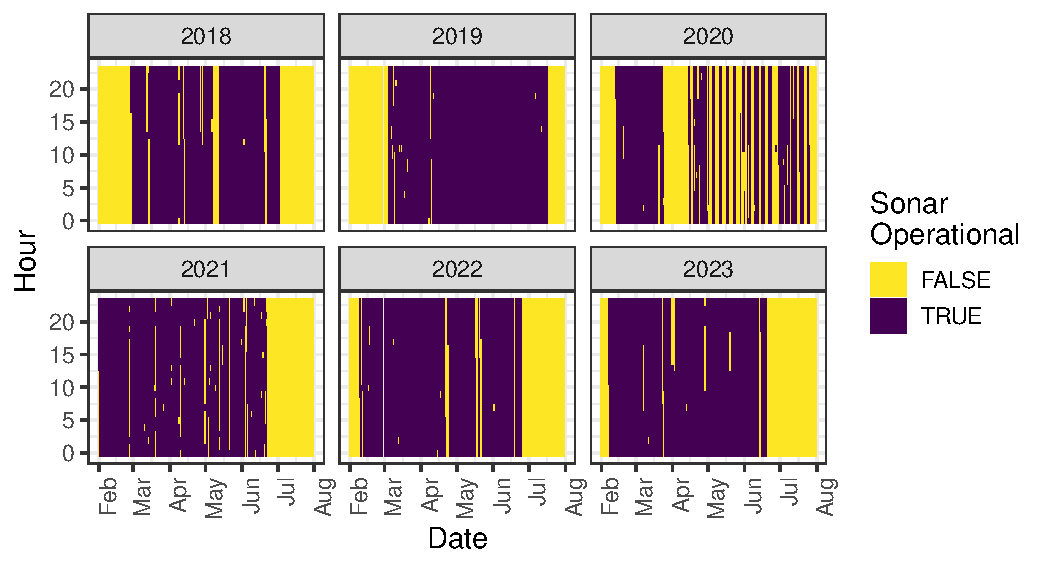
\includegraphics{../figures/op-fig-1.pdf}
\caption{\label{fig:op-fig}Plot of when SONAR was operational (purple) and not (yellow), from Feb 1 through July 31 each year.}
\end{figure}

\begin{figure}
\centering
\includegraphics{../figures/review-fig-1.pdf}
\caption{\label{fig:review-fig}Plot of when SONAR was reviewed (purple) and not (yellow), from Feb 1 through July 31 each year.}
\end{figure}

\FloatBarrier

\hypertarget{data-processing}{%
\subsection{Data Processing}\label{data-processing}}

In 2018 we reviewed both 30-minute files in each hour, for a total of 48 files per 24-hour period. Data review for 2018 was time-consuming and onerous due to the number of fish milling in front of the SONAR, and we were only able to review 22\% of the recorded SONAR imagery over the season (Table \ref{tab:op-rev}). Because of the immense quantity of SONAR files, and the amount of time it took to process and review each 30-minute file, in 2019 we initiated a subsampling design to enable the project team to review portions of nearly every day in the entire period of steelhead passage. In 2019 - 2022 the first 30 minutes of each hour were processed and reviewed for fish migration. A subset of days was fully reviewed (60 minutes of each hour) to compare fish migration with subsampled data (first 30 minutes of each hour). Another subset of days was double, or triple, reviewed to compare fish counts and lengths among each year's 2 or 3 data reviewers. Table \ref{tab:op-rev} shows what percentage of the hours were reviewed each year, and how much of the steelhead migration season was captured by operational SONAR.

\begin{table}[H]

\caption{\label{tab:op-rev}Number of hours during winter steelhead migration period (Feb 1 - June 15) and what percentage of those hours the SONAR was operational and what percentage of those hours have been reviewed.}
\centering
\begin{tabular}[t]{lrrr}
\toprule
Year & Hours & Operational (\%) & Reviewed (\%)\\
\midrule
2018 & 4,344 & 62.9 & 22.1\\
2019 & 4,343 & 73.5 & 41.3\\
2020 & 4,367 & 63.8 & 36.4\\
2021 & 4,343 & 73.4 & 41.9\\
2022 & 4,343 & 71.0 & 40.5\\
\bottomrule
\end{tabular}
\end{table}

Each reviewed imagery file was processed using Sound Metric's proprietary software ARISFish (v2.6.3 -- v2.8.0). First, raw image files were background subtracted, which removed static objects from the image so that only objects in motion are shown. Then, an echogram was created, which transformed the image into a graph of distance (y-axis) and time (x-axis), so that objects in motion appeared as white ``tracks.'' The echogram enabled the data reviewer to quickly navigate to parts of the image file that contained objects that could be migrating fish. These tracks were then manually viewed alongside the raw image file to determine if the object was a fish to be further investigated.

Fish greater or equal to 45 centimeters (cm) were measured, marked, and counted using the ARISFish software. Forty-five cm was determined to be the minimum length of a potential steelhead, based on captures of steelhead during sampling in the Dungeness River 2014, 2015, and 2017 by the Jamestown S'Klallam Tribe (JSK) (unpublished data, C. Burns). Only fish that completely moved through the SONAR beams were counted; fish that nosed in and out or did not completely move from one side of the beams to the other were not counted. For each fish counted the following data were recorded:

\begin{itemize}
\tightlist
\item
  Date
\item
  Hour of the 30-minute image file (e.g., 14:00, 14:30)
\item
  Time
\item
  Frame
\item
  Direction of travel (upstream or downstream)
\item
  Range (distance from the SONAR)
\item
  Length of the fish in cm
\item
  Data reviewer confidence (1 = extremely confident that the object counted is a fish \(\geq\) 45 cm, 2 = somewhat confident that the object is a fish \(\geq\) 45 cm, 3 = object of interest)
\end{itemize}

If no fish were observed in the 30-minute image file, a line of data with ``NO FISH'' was recorded to indicate that the file was reviewed for fish, but no fish \(\geq\) 45 cm were present. Marked fish were automatically saved within the image file for later error checking; data were also recorded within an Excel spreadsheet for data summarization and analysis.

\hypertarget{data-reviewer-comparison}{%
\subsection{Data Reviewer Comparison}\label{data-reviewer-comparison}}

In several years (2019 - 2022), a subset of SONAR footage was reviewed by all (two or three) of that years' observers (Table \ref{tab:obs-rev-tab}). Within that subset of data, we summed the counts of each observer by date and direction before calculating the correlations between counts of different observers using the Pearson correlation coefficient. One observer (initial AS) was an observer every year, while other observers worked for one or two years only. We combined the daily counts across years when computing the correlation between observers. We also computed separate correlations for upstream and downstream counts.

To compare length measurements, we attempted to group individual observer detections of the same fish. We did this by first grouping fish detected in the same hour period moving in the same direction. If there was more than one fish detected in that group, we assumed that the relative lengths assigned by each observer corresponded to the same fish (i.e.~the smallest observed fish by observer A was also the smallest observed fish by observer B). We then calculated the mean, standard deviation and coefficient of variation (CV) of the length measurements for each fish. Because observer AS was the most experienced, and measured nearly every fish, we also compared other observer length measurements against those by AS and treated the measurements by AS as the benchmark for these comparisons. We summarized those differences with statistics such as mean bias, mean absolute error (MAE), root mean squared error (RMSE) and mean absolute percent error (MAPE).

\begin{table}[!h]

\caption{\label{tab:obs-rev-tab}Number of distinct days, hours and individual fish that were double or triple reviewed each year.}
\centering
\begin{tabular}[t]{rrrr}
\toprule
Year & n Days & n Hours & n Fish\\
\midrule
2019 & 5 & 32 & 54\\
2020 & 6 & 34 & 51\\
2021 & 12 & 65 & 92\\
2022 & 14 & 69 & 116\\
\bottomrule
\end{tabular}
\end{table}

\FloatBarrier

\hypertarget{species-composition-sampling}{%
\subsection{Species Composition Sampling}\label{species-composition-sampling}}

Species composition sampling was conducted weekly, as river conditions allowed, during the period of SONAR operations in 2021 and 2022. A fine monofilament gill net 36 feet wide by 8 feet deep with a 2-inch mesh (4-inch stretch) was drifted through all sampleable habitat in the lower river from RM 3.3 to RM 0.5 (2021) or RM 0.8 (2022). Encountered fish were removed immediately from the net, sedated in a solution of tricaine mesylate (MS-222), and sampled for species, origin, length, sex, scales, and DNA. Captured steelhead were assessed for kelt status.

No regular species composition sampling was conducted in 2018, 2019, or 2020. In 2019, three sampling efforts targeting bull trout were conducted once per week in June at sites throughout the Dungeness and Gray Wolf rivers.

\hypertarget{determining-species}{%
\subsection{Determining Species}\label{determining-species}}

Bull trout are swimming past the sonar unit as well as steelhead, and we needed to parse which fish identified by the sonar were steelhead, and exclude any bull trout. The largest bull trout sampled in any species composition data was 67 cm, so we assumed any fish larger than 67 cm detected on the sonar was a steelhead. We then needed to determine of the fish equal to or less than 67 cm long, which of those are steelhead, and which are something else (e.g.~bull trout, rainbow trout).

We modeled the probability of a fish being a steelhead using fork length and the Julian day of capture from the 2021 and 2022 species composition data. Since we only care about differentiating steelhead from other fish, we grouped resident rainbow and cutthroat trout with bull trout, and then fit a binomial GAM with a logit link, using splines of fork length and Julian day to predict the probability of a fish being a steelhead. We did not restrict the dataset to fish with fork lengths less than 67 cm, because larger fish have information about the shape of the logistic curve.

After fitting this GAM, we predicted the probability of being a steelhead for all fish observed on the sonar that were smaller than or equal to 67 cm, based on their length and Julian day of observation. Any fish with a probability of 50\% or greater we assigned to be a steelhead.

\hypertarget{abundance-estimation}{%
\subsection{Abundance Estimation}\label{abundance-estimation}}

Although data was collected for the 2018 run year, the data quality was insufficient to estimate a steelhead abundance for that year. Because we observed frequent milling behavior at the SONAR site, counts were much higher than subsequent years, and only 29\% of the season was reviewed (Table \ref{tab:pct-ops}), we treated 2018 as a pilot year and did not make an escapement estimate.

\begin{table}[!h]

\caption{\label{tab:pct-ops}Number of half hour periods each year between February and mid-June, how many when the SONAR was operational, how many were reviewed and what percentage it was operational and reviewed, 2018 - 2022.}
\centering
\begin{tabular}[t]{lllrrrll}
\toprule
Year & First Day & Last Day & n Periods & n Operational & n Reviewed & Pct Operational & Pct Reviewed\\
\midrule
2018 & Feb 01 & Jun 15 & 6,478 & 4,711 & 1,866 & 72.7\% & 28.8\%\\
2019 & Feb 01 & Jun 15 & 6,478 & 4,848 & 2,724 & 74.8\% & 42.1\%\\
2020 & Feb 01 & Jun 15 & 6,526 & 4,084 & 2,506 & 62.6\% & 38.4\%\\
2021 & Feb 01 & Jun 15 & 6,478 & 6,070 & 3,463 & 93.7\% & 53.5\%\\
2022 & Feb 01 & Jun 15 & 6,478 & 5,738 & 3,276 & 88.6\% & 50.6\%\\
\bottomrule
\end{tabular}
\end{table}

For 2019 - 2022, SONAR fish targets that were larger than 67 cm or had a greater than 50\% probability of being a steelhead, moved completely through the SONAR beams (direction of travel was upstream or downstream), and had a data reviewer confidence of 1 were included in the final steelhead counts and abundance estimate. Based in part on the species composition data, we determined that the steelhead run on the Dungeness is over by mid-June, so we restricted the steelhead season to SONAR observations or predictions between February 1 and June 15.

To fill in the missing data from periods when the SONAR was not operating or the data had not been reviewed, this dataset was fit with a negative binomial generalized additive model (GAM) with a log link function using hour of day, discharge (from a USGS gauge on the Dungeness River, summarized at the hour time-scale) and Julian day-of-year as covariates. The GAM include a cubic spline for the hour of day, a thin-plate spline for discharge, and a factor spline for day of year, including an interaction between year and day of year. This GAM was then used to predict the upstream and downstream numbers of steelhead during all missing data periods, from February 1 through June 15 each year. This included all half hours when the SONAR was not operational for the entire 30 min, as well as all half hours that were not reviewed.

To combine the upstream and downstream estimates, we made one simplifying assumption related to kelting behavior. Prior to May 15, we subtracted the total estimate of downstream moving fish from the total estimate of upstream moving fish. This is to prevent fish that are milling (moving upstream, then downstream, then upstream again) from being double counted. After May 15, we ignored downstream moving fish and only estimated upstream moving fish, under the assumption that downstream moving fish are steelhead kelts that have spawned and therefore should not be subtracted from our escapement estimates. Obviously, there may be kelts prior to May 15, and there may be milling fish after that date, but our assumption is that the number of downstream moving kelts prior to that date equals the number of downstream milling fish after that date.

\hypertarget{comparison-with-redd-based-estimates}{%
\subsubsection{Comparison with Redd-Based Estimates}\label{comparison-with-redd-based-estimates}}

The Jamestown S'Klallam Tribe has conducted redd surveys for steelhead on the Dungeness for many years. In most years, rising flows and increased turbidity close the river to surveyors before the end of steelhead spawning season. However, in 2015, conditions allowed for surveys to be completed through the end of the spawning season. For other years, the number of redds surveyed is expanded by the proportion of total redds observed in 2015 up to the date of the last survey in that year. These estimates of total redds are then expanded to spawners by multiplying by a fish / redd constant of 1.62. We compared the SONAR-based estimates of steelhead escapement to the redd-based estimates of steelhead spawners for 2019, 2021 and 2022. Due to COVID, no redd surveys were conducted in 2020, so no redd-based estimate is available.

\FloatBarrier

\hypertarget{results}{%
\section{Results}\label{results}}

\hypertarget{data-reviewer-comparison-1}{%
\subsection{Data Reviewer Comparison}\label{data-reviewer-comparison-1}}

After summing the counts across days when each pair of observers reviewed the same footage, Table \ref{tab:obs-totals} shows the total counts by year and direction (upstream vs.~downstream) for each observer. Generally, the upstream counts are very well aligned, and the downstream counts are close although they show more observer-to-observer variability than upstream counts.

\begin{table}[!h]

\caption{\label{tab:obs-totals}Total counts of steelhead by direction and year for each observer pair during days when both observers were counting.}
\centering
\begin{tabular}[t]{rlrrrrrr}
\toprule
Year & Direction & AS & BC & BT & CS & GB & JG\\
\midrule
2019 &  & 38 & 38 & - & - & - & -\\
\cmidrule{1-1}
\cmidrule{3-8}
2019 &  & - & 38 & - & - & - & 37\\
\cmidrule{1-1}
\cmidrule{3-8}
2019 &  & 38 & - & - & - & - & 37\\
\cmidrule{1-1}
\cmidrule{3-8}
2020 &  & 31 & - & 32 & - & - & -\\
\cmidrule{1-1}
\cmidrule{3-8}
2021 &  & 14 & - & 13 & - & - & -\\
\cmidrule{1-1}
\cmidrule{3-8}
2021 &  & 26 & - & - & 26 & - & -\\
\cmidrule{1-1}
\cmidrule{3-8}
2021 &  & - & - & 3 & 3 & - & -\\
\cmidrule{1-1}
\cmidrule{3-8}
2022 &  & 47 & - & - & 48 & - & -\\
\cmidrule{1-1}
\cmidrule{3-8}
2022 &  & 54 & - & - & - & 40 & -\\
\cmidrule{1-1}
\cmidrule{3-8}
2022 & \multirow{-10}{*}{\raggedright\arraybackslash Upstream} & - & - & - & 46 & 32 & -\\
\cmidrule{1-8}
\midrule
2019 &  & 6 & 7 & - & - & - & -\\
\cmidrule{1-1}
\cmidrule{3-8}
2019 &  & - & 7 & - & - & - & 5\\
\cmidrule{1-1}
\cmidrule{3-8}
2019 &  & 9 & - & - & - & - & 7\\
\cmidrule{1-1}
\cmidrule{3-8}
2020 &  & 15 & - & 12 & - & - & -\\
\cmidrule{1-1}
\cmidrule{3-8}
2021 &  & 19 & - & 19 & - & - & -\\
\cmidrule{1-1}
\cmidrule{3-8}
2021 &  & 24 & - & - & 20 & - & -\\
\cmidrule{1-1}
\cmidrule{3-8}
2021 &  & - & - & 6 & 1 & - & -\\
\cmidrule{1-1}
\cmidrule{3-8}
2022 &  & 20 & - & - & 12 & - & -\\
\cmidrule{1-1}
\cmidrule{3-8}
2022 &  & 24 & - & - & - & 13 & -\\
\cmidrule{1-1}
\cmidrule{3-8}
2022 & \multirow{-10}{*}{\raggedright\arraybackslash Downstream} & - & - & - & 9 & 6 & -\\
\bottomrule
\end{tabular}
\end{table}

The correlation coefficient between each pair of observers, by direction, is show in Table \ref{tab:obs-corr}. Except for observer GB, Correlations for upstream moving fish were all greater than 0.95, while the correlation coefficients for downstream moving fish ranged from -0.25 to 0.87. Several of the weakest correlations did correspond with lower numbers of observed fish.

\begin{table}[!h]

\caption{\label{tab:obs-corr}Correlation (r) between daily counts of upstream and downstream moving fish for periods that were reviewed by pairs of observers. The total number of days when each pair reviewed SONAR data is shown, as well as the total number of fish observed by each observer.}
\centering
\begin{tabular}[t]{lllrrrr}
\toprule
Direction & Obs 1 & Obs 2 & N Days & Obs 1 Fish & Obs 2 Fish & r\\
\midrule
Upstream & AS & JG & 5 & 38 & 37 & 0.998\\
Upstream & BC & JG & 5 & 38 & 37 & 0.995\\
Upstream & AS & BC & 5 & 38 & 38 & 0.991\\
Upstream & AS & BT & 11 & 45 & 45 & 0.976\\
Upstream & AS & CS & 15 & 73 & 74 & 0.951\\
Upstream & CS & GB & 8 & 46 & 42 & 0.495\\
Upstream & AS & GB & 10 & 54 & 42 & 0.404\\
\midrule
Downstream & AS & BC & 3 & 6 & 7 & 0.866\\
Downstream & AS & BT & 10 & 34 & 31 & 0.863\\
Downstream & AS & CS & 14 & 44 & 33 & 0.654\\
Downstream & AS & GB & 7 & 24 & 13 & 0.541\\
Downstream & BC & JG & 3 & 7 & 7 & 0.500\\
Downstream & AS & JG & 4 & 9 & 7 & 0.174\\
Downstream & CS & GB & 5 & 9 & 13 & -0.250\\
\bottomrule
\end{tabular}
\end{table}

For fish observed by multiple observers, the CVs of those multiple length measurements are displayed in Figure \ref{fig:cv-lgth-hist}. The mean CV of length measurements for upstream moving fish was 0.06, while it was 0.09 for downstream moving fish. 95\% of the upstream CVs were smaller than 0.15 (considered a reference point for precise measurements), while 84\% of the downstream CVs met this criterion.

\begin{figure}
\centering
\includegraphics{../figures/cv-lgth-hist-1.pdf}
\caption{\label{fig:cv-lgth-hist}Coefficient of variation (CV) of length measurements for individual fish across multiple observers, colored by year and faceted by direction of movement. Dashed lines indicate the mean CV for that group, while the solid black line is a reference of 0.15.}
\end{figure}

Histograms of length measurement bias, relative to observer AS, are shown in Figure \ref{fig:lgth-comp-fig}. Summary statistics of the same comparison are depicted in Table \ref{tab:lgth-comp-tab}. All observers had larger variability in their measurements of downstream moving fish compared to observer AS, as seen in RMSE, MAE and MAPE values. Two observers (BT and GB) had a positive mean bias relative to observer AS for upstream fish and BT also had a positive mean bias for downstream fish, meaning they often measured the same fish as being slightly larger than AS. The other observers had negative mean bias, meaning they measured the same fish as being smaller compared to observer AS. This was more pronounced for downstream moving fish, up to an mean difference of nearly -12.4 cm per fish for observer BC (although that observer only measured four downstream fish).

The mean absolute percent error (MAPE) ranged from 6.7 - 12.3\% for upstream moving fish and from 8.9 - 18.2\% for downstream moving fish. To put that on the scale of fish lengths (centimeters), the root mean square error (RMSE) ranged from 6.7 - 9.6 cm for upstream moving fish and 6.8 - 17 cm for downstream moving fish.

\begin{figure}
\centering
\includegraphics{../figures/lgth-comp-fig-1.pdf}
\caption{\label{fig:lgth-comp-fig}Histograms and density plots showing the bias of length measurements, relative to observer AS, colored by observer and faceted by direction and year.}
\end{figure}

\begin{table}[!h]

\caption{\label{tab:lgth-comp-tab}Summary statistics comparing length measurements of different observers with those made by observer AS.}
\centering
\begin{tabular}[t]{llrrrrr}
\toprule
Direction & Observer & N Fish & Mean Bias & RMSE & MAE & MAPE\\
\midrule
Upstream & CS & 63 & -1.1 & 7.8 & 5.7 & 8.9\\
Upstream & BT & 41 & 1.5 & 8.3 & 5.7 & 9.1\\
Upstream & JG & 37 & -6.3 & 8.3 & 6.8 & 9.3\\
Upstream & BC & 36 & -2.3 & 6.7 & 4.9 & 6.7\\
\midrule
Upstream & GB & 29 & 1.9 & 9.6 & 7.4 & 12.3\\
Downstream & BT & 24 & 1.5 & 9.7 & 7.4 & 12.6\\
Downstream & CS & 23 & -4.4 & 6.8 & 6.0 & 8.9\\
Downstream & GB & 7 & -2.0 & 15.1 & 12.4 & 18.2\\
Downstream & JG & 5 & -7.4 & 12.1 & 10.7 & 13.0\\
Downstream & BC & 4 & -12.4 & 17.0 & 13.0 & 14.5\\
\bottomrule
\end{tabular}
\end{table}

\FloatBarrier

\hypertarget{species-composition}{%
\subsection{Species Composition}\label{species-composition}}

Thirty-three species composition sampling events were conducted between early February and late June across 2021 and 2022. Steelhead and bull trout were the primary species encountered during sampling. The majority of captured steelhead were natural-origin; three hatchery-origin steelhead were captured in early April 2021, and three hatchery-origin steelhead were captured in 2022 - two in mid-March and one in late May. Steelhead kelts were encountered starting in early June 2021 and in May 2022 (Table \ref{tab:spp-cnts-date}). From the species composition netting, there are 92 fish to use in this model. The lengths of these fish can be seen in Figure \ref{fig:fl-hist}.

\begin{longtable}[t]{cc>{\centering\arraybackslash}p{1.5cm}>{\centering\arraybackslash}p{1.5cm}>{\centering\arraybackslash}p{1.5cm}>{\centering\arraybackslash}p{1.5cm}>{\centering\arraybackslash}p{1.5cm}>{\centering\arraybackslash}p{1.5cm}}
\caption{\label{tab:spp-cnts-date}Counts of species encountered during species composition sampling in the lower Dungeness River in 2021 and 2022, differentiating between marked or clipped steelhead (AD) and unmarked steelhead (UM) and including steelhead kelts.}\\
\toprule
Year & Date & Bull Trout & Resident Rainbow & Cutthroat & Steelhead (UM) & Steelhead (AD) & Steelhead Kelt\\
\midrule
\endfirsthead
\caption[]{\label{tab:spp-cnts-date}Counts of species encountered during species composition sampling in the lower Dungeness River in 2021 and 2022, differentiating between marked or clipped steelhead (AD) and unmarked steelhead (UM) and including steelhead kelts. \textit{(continued)}}\\
\toprule
Year & Date & Bull Trout & Resident Rainbow & Cutthroat & Steelhead (UM) & Steelhead (AD) & Steelhead Kelt\\
\midrule
\endhead

\endfoot
\bottomrule
\endlastfoot
 & Feb 17 & 1 & 0 & 0 & 0 & 0 & 0\\
\cmidrule{2-8}\nopagebreak
 & Feb 22 & 0 & 0 & 0 & 2 & 0 & 0\\
\cmidrule{2-8}\nopagebreak
 & Feb 25 & 0 & 0 & 0 & 2 & 0 & 0\\
\cmidrule{2-8}\nopagebreak
 & Feb 26 & 0 & 0 & 0 & 1 & 0 & 0\\
\cmidrule{2-8}\nopagebreak
 & Mar 03 & 0 & 0 & 0 & 1 & 0 & 0\\
\cmidrule{2-8}\nopagebreak
 & Mar 04 & 1 & 0 & 0 & 0 & 0 & 0\\
\cmidrule{2-8}\nopagebreak
 & Mar 17 & 0 & 0 & 0 & 1 & 0 & 0\\
\cmidrule{2-8}\nopagebreak
 & Mar 18 & 0 & 0 & 0 & 1 & 0 & 0\\
\cmidrule{2-8}\nopagebreak
 & Mar 25 & 0 & 0 & 0 & 2 & 0 & 0\\
\cmidrule{2-8}\nopagebreak
 & Mar 26 & 0 & 1 & 0 & 1 & 0 & 0\\
\cmidrule{2-8}\nopagebreak
 & Apr 01 & 1 & 0 & 0 & 1 & 1 & 0\\
\cmidrule{2-8}\nopagebreak
 & Apr 06 & 2 & 0 & 0 & 0 & 0 & 0\\
\cmidrule{2-8}\nopagebreak
 & Apr 07 & 0 & 0 & 0 & 2 & 0 & 0\\
\cmidrule{2-8}\nopagebreak
 & Apr 08 & 0 & 0 & 0 & 4 & 2 & 0\\
\cmidrule{2-8}\nopagebreak
 & Apr 14 & 0 & 0 & 0 & 4 & 0 & 0\\
\cmidrule{2-8}\nopagebreak
 & Apr 15 & 3 & 0 & 0 & 0 & 0 & 0\\
\cmidrule{2-8}\nopagebreak
 & Apr 16 & 1 & 0 & 0 & 1 & 0 & 0\\
\cmidrule{2-8}\nopagebreak
 & Apr 28 & 0 & 0 & 0 & 1 & 0 & 0\\
\cmidrule{2-8}\nopagebreak
 & May 05 & 0 & 0 & 0 & 1 & 0 & 0\\
\cmidrule{2-8}\nopagebreak
\multirow{-20}{*}{\centering\arraybackslash 2021} & Jun 08 & 4 & 2 & 0 & 1 & 0 & 1\\
\cmidrule{1-8}\pagebreak[0]
\midrule
\textbf{2021} & \textbf{Total} & \textbf{13} & \textbf{3} & \textbf{0} & \textbf{26} & \textbf{3} & \textbf{1}\\
\cmidrule{1-8}\pagebreak[0]
 & Feb 02 & 3 & 0 & 1 & 0 & 0 & 0\\
\cmidrule{2-8}\nopagebreak
 & Feb 15 & 1 & 0 & 0 & 0 & 0 & 0\\
\cmidrule{2-8}\nopagebreak
 & Feb 22 & 0 & 0 & 0 & 2 & 0 & 0\\
\cmidrule{2-8}\nopagebreak
 & Mar 09 & 1 & 0 & 0 & 1 & 1 & 0\\
\cmidrule{2-8}\nopagebreak
 & Mar 16 & 0 & 0 & 0 & 2 & 1 & 0\\
\cmidrule{2-8}\nopagebreak
 & Mar 23 & 1 & 0 & 0 & 1 & 0 & 0\\
\cmidrule{2-8}\nopagebreak
 & Mar 30 & 0 & 0 & 0 & 2 & 0 & 0\\
\cmidrule{2-8}\nopagebreak
 & Apr 07 & 1 & 0 & 0 & 3 & 0 & 0\\
\cmidrule{2-8}\nopagebreak
 & Apr 19 & 2 & 0 & 0 & 7 & 0 & 0\\
\cmidrule{2-8}\nopagebreak
 & May 04 & 2 & 0 & 0 & 6 & 0 & 4\\
\cmidrule{2-8}\nopagebreak
 & May 20 & 2 & 0 & 0 & 2 & 1 & 2\\
\cmidrule{2-8}\nopagebreak
 & Jun 01 & 2 & 0 & 0 & 1 & 0 & 1\\
\cmidrule{2-8}\nopagebreak
\multirow{-13}{*}{\centering\arraybackslash 2022} & Jun 22 & 1 & 0 & 0 & 0 & 0 & 0\\
\cmidrule{1-8}\pagebreak[0]
\midrule
\textbf{2022} & \textbf{Total} & \textbf{16} & \textbf{0} & \textbf{1} & \textbf{27} & \textbf{3} & \textbf{7}\\*
\end{longtable}

\begin{figure}
\centering
\includegraphics{../figures/fl-hist-1.pdf}
\caption{\label{fig:fl-hist}Histogram of forklengths, colored by species. Dashed lines are the overlap range between steelhead and other species.}
\end{figure}

\hypertarget{determining-species-1}{%
\subsection{Determining Species}\label{determining-species-1}}

The impacts of Julian day and fork length on the probability of a fish being a steelhead are displayed in Figure \ref{fig:spp-pred}. Generally, larger fish have a greater chance of being a steelhead, but the exact break point of length (i.e.~50\% probability of being a steelhead) shifts over the course of the season.

Fish greater than 67 cm were deemed steelhead, regardless of the Julian day of year they were observed. Fish less than or equal to 67 cm were deemed steelhead if the predicted probability of being a steelhead from our GAM model was greater than or equal to 50\%. The number of fish within each category is shown in Table \ref{tab:pred-sthd-gam}.

\begin{figure}
\centering
\includegraphics{../figures/spp-pred-1.pdf}
\caption{\label{fig:spp-pred}Julian day and fork length of each fish detected on SONAR, colored by the predicted probability of being a steelhead. Size of the point corresponds to the precision of the predicted probability (larger points indicate greater precision). Dark line indicates the 50\% probability of being a steelhead. Dashed horizontal lines depict 45 and 67 cm lengths for reference.}
\end{figure}

\begin{table}[!h]

\caption{\label{tab:pred-sthd-gam}Number of fish observed moving downstream or upstream (n Fish), less than or greater than 67 cm, and whether they were likely (> 50\% probability) to be a steelhead. Totals within each movement and size group are shown (n Sthd) as well as totals for each year by direction (Total Sthd).}
\centering
\resizebox{\linewidth}{!}{
\begin{tabular}[t]{lrrrrrrr>{}r}
\toprule
\multicolumn{1}{c}{} & \multicolumn{1}{c}{} & \multicolumn{3}{c}{<= 67 cm} & \multicolumn{3}{c}{> 67 cm} & \multicolumn{1}{c}{} \\
\cmidrule(l{3pt}r{3pt}){3-5} \cmidrule(l{3pt}r{3pt}){6-8}
Direction & Year & n Fish & Likely Sthd & n Sthd & n Fish & Likely Sthd & n Sthd & Total Sthd\\
\midrule
 & 2019 & 268 & 136 & 136 & 477 & 477 & 477 & \textbf{613}\\
\cmidrule{2-9}
 & 2020 & 416 & 280 & 280 & 414 & 414 & 414 & \textbf{694}\\
\cmidrule{2-9}
 & 2021 & 266 & 148 & 148 & 496 & 473 & 496 & \textbf{644}\\
\cmidrule{2-9}
\multirow{-4}{*}{\raggedright\arraybackslash Upstream} & 2022 & 450 & 292 & 292 & 284 & 281 & 284 & \textbf{576}\\
\cmidrule{1-9}
 & 2019 & 95 & 50 & 50 & 207 & 207 & 207 & \textbf{257}\\
\cmidrule{2-9}
 & 2020 & 234 & 145 & 145 & 119 & 119 & 119 & \textbf{264}\\
\cmidrule{2-9}
 & 2021 & 205 & 110 & 110 & 214 & 210 & 214 & \textbf{324}\\
\cmidrule{2-9}
\multirow{-4}{*}{\raggedright\arraybackslash Downstream} & 2022 & 198 & 120 & 120 & 109 & 108 & 109 & \textbf{229}\\
\bottomrule
\end{tabular}}
\end{table}

\FloatBarrier

\hypertarget{abundance-estimation-1}{%
\subsection{Abundance Estimation}\label{abundance-estimation-1}}

The estimated marginal effects of various covariates on the expected number of upstream and downstream moving fish are shown in Figures \ref{fig:up-marg} and \ref{fig:down-marg} respectively. For both directions, the model indicates that a greater number of steelhead will move during the night, especially in the late evening, compared to the daytime, and more will move when discharge flows are near 600 cfs. There is also a clear effect of day-of-year, with upstream numbers peaking near the beginning of April, while downstream numbers peak near the beginning of May, with some year-to-year variability in that run-timing curve.

Estimates of early, late, and total annual escapement of winter steelhead are shown in Table \ref{tab:year-tab}.

\begin{table}[!h]

\caption{\label{tab:year-tab}Annual estimates of winter steelhead in the early (upstream - downstream) and late (upstream only) periods as well as total upstream escapement to the Dungeness River between Feb 1 and June 15.}
\centering
\resizebox{\linewidth}{!}{
\begin{tabular}[t]{l>{}rrrr>{}rrrr>{}rrrr}
\toprule
\multicolumn{1}{c}{} & \multicolumn{4}{c}{Early} & \multicolumn{4}{c}{Late} & \multicolumn{4}{c}{Total} \\
\cmidrule(l{3pt}r{3pt}){2-5} \cmidrule(l{3pt}r{3pt}){6-9} \cmidrule(l{3pt}r{3pt}){10-13}
Year & Estimate & SE & Low CI & Upp CI & Estimate & SE & Low CI & Upp CI & Estimate & SE & Low CI & Upp CI\\
\midrule
2019 & \textbf{762} & 146.9 & 658 & 1,160 & \textbf{152} & 7.3 & 140 & 168 & \textbf{913} & 147.2 & 808 & 1,317\\
2020 & \textbf{961} & 43.1 & 878 & 1,045 & \textbf{140} & 17.5 & 112 & 181 & \textbf{1,101} & 47.1 & 1,012 & 1,196\\
2021 & \textbf{579} & 8.9 & 562 & 597 & \textbf{67} & 4.8 & 59 & 78 & \textbf{646} & 10.8 & 626 & 668\\
2022 & \textbf{610} & 11.4 & 587 & 629 & \textbf{138} & 8.3 & 123 & 156 & \textbf{747} & 14.8 & 719 & 776\\
\bottomrule
\end{tabular}}
\end{table}

\begin{figure}
\centering
\includegraphics{../figures/up-marg-1.pdf}
\caption{\label{fig:up-marg}Marginal effects for upstream-moving fish as estimated by the GAM for hour of day (A), discharge (B), and Julian day of year (C). Shaded areas indicated 95\% confidence intervals.}
\end{figure}

\begin{figure}
\centering
\includegraphics{../figures/down-marg-1.pdf}
\caption{\label{fig:down-marg}Marginal effects for downstream-moving fish as estimated by the GAM for hour of day (A), discharge (B), and Julian day of year (C). Shaded areas indicated 95\% confidence intervals.}
\end{figure}

\FloatBarrier

\hypertarget{comparison-with-redd-based-estimates-1}{%
\subsubsection{Comparison with Redd-Based Estimates}\label{comparison-with-redd-based-estimates-1}}

Comparisons between redd-based estimates and SONAR-based estimates can be seen in Table \ref{tab:redd-tab} and Figure \ref{fig:redd-fig}. In the three years with comparable estimates, SONAR-based estimates were significantly higher than redd-based ones each year. In fact, the redd-based estimates were much closer to the number of steelhead counted on SONAR, before accounting for periods when the SONAR was not operating or the footage was not reviewed. The redd-based estimates did not fall within the 95\% confidence intervals of the SONAR-based estimates.

\begin{table}[!h]

\caption{\label{tab:redd-tab}Annual estimates of upstream escapement of winter steelhead to the Dungeness River between Feb 1 and June 15, including counts of observed fish (from SONAR) and redd-based estimate of spawners.}
\centering
\begin{tabular}[t]{lrrrrrr}
\toprule
Year & SONAR Est. & SE & Low CI & Upp CI & SONAR Obs Sthd. & Redd Est.\\
\midrule
2019 & 913 & 147 & 807.9 & 1,317 & 420 & 467\\
2020 & 1,101 & 47 & 1,012.2 & 1,196 & 453 & -\\
2021 & 646 & 11 & 626.4 & 668 & 356 & 329\\
2022 & 747 & 15 & 718.7 & 776 & 405 & 386\\
\bottomrule
\end{tabular}
\end{table}

\begin{figure}
\centering
\includegraphics{../figures/redd-fig-1.pdf}
\caption{\label{fig:redd-fig}Annual estimates of upstream escapement of winter steelhead to the Dungeness River between Feb 1 and June 15, including counts of observed fish (from SONAR) and redd-based estimate of spawners.}
\end{figure}

\FloatBarrier
\newpage

\hypertarget{discussion}{%
\section{Discussion}\label{discussion}}

We used SONAR to make annual estimates of winter steelhead on the Dungeness River for spawn years 2019 - 2022. To do so, we needed to collect and utilize independent species composition data, and develop an analysis technique that allowed us to estimate passage during periods when the SONAR was not operable or the video had not been reviewed. In addition, analyzing these initial years of data has prompted several observations worth mentioning.

First, SONAR location is a crucial component of a successful SONAR project. After observing the fish behavior at the initial location in 2018, we moved the SONAR to a habitat unit that was more of a run, and more conducive to fish actively migrating through rather than milling around. In addition to fish behavior at the site, access and security are important considerations. After we moved the SONAR site slightly upstream in 2019, and deployed the unit from a fixed platform on the bank, it was much easier for the team to check on and make adjustments to the unit. The 2019-2022 site is also located on WDFW property, enabling a direct power source, and an on-site staff trailer for security and comfort in bad weather.

In addition to the location, several factors in 2018 led to unrealistic estimates of escapement. The amount of SONAR imagery that was not reviewed in 2018 was much higher than in other years (Figures \ref{fig:op-fig} and \ref{fig:review-fig} and Table \ref{tab:pct-ops}). Additionally, the counts of both upstream and downstream moving fish were much higher in 2018, presumably due in part to more milling behavior at that site. The mean count of upstream moving fish in 2018 in a half-hour period was 1.02, while it ranged from 0.24 - 0.35 in 2019 - 2022. For downstream moving fish it was a mean of 0.70 in 2018, and a range of 0.1 - 0.15 in 2019 - 2022. Due to these reasons, we made the decision to treat 2018 as a pilot year and did not make a SONAR-based escapement estimate, and instead utilize the lessons learned from that year to improve operations in subsequent years.

Second, the variability between observers was relatively small. The total counts between pairs of observers each year were very similar, especially for upstream moving fish (Table \ref{tab:obs-totals}). The coefficient of variation among different observers' length measurements was quite small, suggesting good consistency across observers. It should be noted that we matched up which fish each observer measured in such a way as to minimize observer-to-observer differences for multiple fish observed in the same half-hour period. The overall bias in measurements, compared to observer AS, was quite low, but not zero. This could have an impact on whether a fish is predicted to be a steelhead or not, since length is a determining covariate in the species prediction model. However, Figure \ref{fig:lgth-comp-fig} suggests that there are differences in length measurements in both the positive and negative direction, so the impact on steelhead counts should be minimal.

Third, how to best deal with steelhead kelts is an open question. For fish that move upstream, downstream, and upstream again before spawning, we would like to subtract the downstream counts from the upstream counts, to avoid double-counting the same fish. However, steelhead that kelt may be observed moving upstream and again moving downstream, and we would not like those counts to cancel each other out. Currently, we are sidestepping this issue by assuming that the number of kelts detected prior to May 15 is equal to the number of downstream milling detections after that date. However, that date is at best an educated guess which could lead to bias in our estimates in one direction or the other. Continued investigation of this issue is warranted, perhaps by more closely examining the species composition data for kelting behavior (or changing the species composition sampling to better target kelts) or by analyzing metrics such as the upstream:downstream count ratios through the season, to determine if there is a pattern that could guide what that equilibrium date should be.

Finally, the species composition data raised a few issues for future consideration. A few bull trout were captured multiple times in the same pool during species composition netting, suggesting that the species composition sampling may be sampling not just fish that are moving, but also fish that may be holding (i.e.~not moving past the SONAR). Whether this actually impacts the predictions of species based on size and Julian day is unclear. In addition, the current methods cannot account for potential differences in what hour of the day certain species are more or less likely to move. If steelhead are more likely to move at night, as suggested by the hour of day co-variate in our model, compared to other species, we would want to incorporate hour of day into our species prediction. Without a different study design for species composition, we are unable to address this question. However, it seems reasonable to assume that steelhead and bull trout have similar behavior with regards to movement and time of day.

The SONAR-based estimates of steelhead escapement were significantly greater than redd-based estimates for the three years we could makes comparisons. Although the two estimates are focused on slightly different life-stages (SONAR-based estimates are focused on pre-spawn steelhead, while redd-based estimates focus on spawners), and some steelhead may experience pre-spawn mortality, we would not expect that to explain the large differences between the two estimates. We hypothesize that the redd-based estimate could be biased low because steelhead redds are more difficult to see, and often observed imperfectly (Murdoch et al. 2018), leading to an under-count of redds. In addition, perhaps not all of steelhead spawning habitat was surveyed for redds. In fact, the Grey Wolf River and upper Dungeness are difficult to access, and due to their high gradients, must be surveyed at lower flows than the lower basin, resulting in few surveys per season, and the potential to miss redds. Another reason for this could be because the fish / redd number used, 1.62, is too low. Finally, the year that redd expansions are based on, 2015, was an abnormally low water year, and may not reflect spawn timing in average water years. Alternatively, the SONAR-based estimate could be biased high if the date we chose to stop subtracting downstream moving fish was too early, or if our species composition model identified too many non-steelhead fish as steelhead. It should be noted that the SONAR-based estimates consistently tracked the redd-based estimates (redd-based estimates were on average 51.2 \% of the SONAR-based estimates), suggesting a consistent bias between the two.

\hypertarget{recommendations}{%
\subsection{Recommendations}\label{recommendations}}

In the future, we recommend setting the SONAR unit up earlier in the year, before the steelhead start moving into the Dungeness. Even in 2021, when the SONAR was deployed starting February 1, there was still one steelhead detected on that date, suggesting the run may begin sooner than that. If the SONAR is deployed earlier, then we would also recommend that the species composition sampling begin at the same point in the year that the SONAR is deployed, to ensure that we can identify when steelhead (as opposed to other species) are moving in the Dungeness. After a few years of deploying quite early, we may begin to move that deployment date later with a firmer understanding of when the run starts.

We also recommend investigating the use of image recognition software and machine learning processing to help automate the review of SONAR images. Technicians are required to spend a substantial amount of time reviewing SONAR video, and if that could be reduced it would have multiple benefits. First, cutting hours of tedious review time could potentially be cost-effective, and make the data available for analysis sooner. Second, it would make the counts more reproducible and less subject to an individual observer's skill and experience. Finally, by automating the review process there would no longer be a need to selectively choose which periods to review (e.g.~first 30 minutes of every hour). Instead, counts could be obtained for the entire period the SONAR is deployed, reducing the reliance on estimates for periods with missing data.

Additionally, we recommend considering study design changes to the species composition sampling to answer the questions we have with these data. We could consider constraining the species composition sampling closer to the SONAR site to attempt to capture only fish actively migrating, and not fish that are holding. We also recommend testing whether time of day affects the species composition by doing some sampling sets in the late afternoon and evening.

\hypertarget{acknowledgements}{%
\section{Acknowledgements}\label{acknowledgements}}

Andrew Simmons, Dan Gorze, Jayson Gallatin, Brent Trim, and Greg Boecker of WDFW operated, maintained, and reviewed SONAR imagery data. Calvin Stokes also reviewed SONAR imagery. Peter Topping provided project support and advice. Kathryn Sutton led weekly species composition sampling with the help of many volunteers including Calvin Stokes, Jenni Whitney, Scott Williams, Jeff Gufler, David Thomas, Jacob Portney, Caleb Owen, and Kayla Own of WDFW, Chris Burns, Jarrett Burns, Casey Allen, and Aaron Brooks of the Jamestown S'Klallam Tribe, Dave Shreffler of Shreffler and Associates, Keith Denton of Keith Denton and Associates, and Roger Peters, Roger Tabor, Greg Byford, Evan Lewis, Jakob Bengelink, and Jack Brill of the U.S. Fish and Wildlife Service.

\hypertarget{literature-cited}{%
\section{Literature Cited}\label{literature-cited}}

\hypertarget{refs}{}
\begin{CSLReferences}{1}{0}
\leavevmode\vadjust pre{\hypertarget{ref-Ford2011}{}}%
Ford, M. J., A. Albaugh, K. Barnas, T. D. Cooney, J. Cowen, J. J. Hard, R. G. Kope, M. M. McClure, P. McElhany, J. M. Myers, and others. 2011. Status review update for {Pacific} salmon and steelhead listed under the {Endangered Species Act}: {Pacific Northwest}. {NOAA Fisheries}, NMFS-NWFSC-113, {Northwest Fisheries Science Center Seattle}.

\leavevmode\vadjust pre{\hypertarget{ref-Murdoch2018}{}}%
Murdoch, A. R., C. J. Herring, C. H. Frady, K. See, and C. E. Jordan. 2018. Estimating observer error and steelhead redd abundance using a modified {Gaussian} area-under-the-curve framework. Canadian Journal of Fisheries and Aquatic Sciences 75(12):2149--2158.

\leavevmode\vadjust pre{\hypertarget{ref-Myers2015}{}}%
Myers, J. M., J. J. Hard, E. J. Connor, R. A. Hayman, R. G. Kope, G. Lucchetti, A. R. Marshall, G. R. Pess, and B. E. Thomson. 2015. Identifying historical populations of steelhead within the {Puget Sound} distinct population segment. {U.S. Department of Commerce}, NMFS- NWFSC-128.

\leavevmode\vadjust pre{\hypertarget{ref-NWFSC2015}{}}%
Northwest Fisheries Science Center. 2015. Status review update for {Pacific} salmon and steelhead listed under the {Endangered Species Act}: {Pacific Northwest}. {NOAA Fisheries}, {Northwest Fisheries Science Center Seattle}.

\end{CSLReferences}

\end{document}
